\documentclass[12pt]{article}
\usepackage{graphicx}

\author{Samuel Young}
\title{EXAM  II}
\date{Thursday ,April 26th, 2018}
\begin{document}

\maketitle
\begin{itemize}
	\item
\part{1.A Understand the question that is being asked.}
  I started by reading "Global mapping of MtrA-binding sites links MtrA to regulation of its targets in \textit{Mycobacterium tuberculosis}" for better insight.  In  the reading of the meat of the article states that rpfA, rpoB, relF, and rpfB, rpfc  promoter regions. It seems that  have of found the promoters regions for  the MtrA. They found a MtrA-binding site of the sequence upstream. Rv2524c and Rv3246c (chatterjee et. al,102). In the article, they empolyed using MEME software to find the promoters in both regions of rpfA and rpfC(chatterjee et. al, 102). I did similar something similar I used memes to find upwards of 5 sequences that had some likelyhood of PSSM  similarity to most of the groups. I also removed a majority of the unneed DNA locations and only kept in the DNA binding promoters to our target gene  an the hypotheicial genes because I was unsure of what there functionality was.I then download the logos from memes. 
\part{1.B back to the salts mines}
  In line thriteen, there seems to be a large amount a majority of them that where G and it likely  in line 13 there appears to be 2 A that came up in my assumption that I made this actaul frequency was 1 to 21 G for this line. In line six and seventeen they appear t  have some what of a similar sizes  of C and A's being used  In this one I forgot to estimate the size for these one but I know the right size for 6  is  C eighteen  to four A and the size fo 17 was  C ninteen and A of three. So I used information in py to  generate the graphs
\part{1.C eating all the salt}
At first I was trying to use the find function on firefox and begin with a base sequecence but once that end up not panning out I was only able to obtain  get  3 or  6 letters in to it before thing kept on hitting the bells. I could always consider trying to run against a phoylogneic tree to find the possible sites of similarity.
	\item
\part{2.A}
 There are just about 72 possible ALL and AML data point within the data set. There are a total 47 ALL in the dataset  and 25 of the AML in the same data set. So the genes are the rows and the columns are the patients. So first I did a wordcount on the file to see how many rows there are and then minus the 7219-1 to get a close approximation to the numbers there are 72* 7218 differnet genes to look at for the data set.

\part{2.B}
		I orignial thought that there were at least 500-1000 of these genes had a greater than or equal to 2.000 p-value with a degree of freedom of 60, It was any assumption, made based on t-chart that I made base on the data that was given. But considering there are to different sigigincat factor that can still be held true. I was solely basing on one data set when what i should have of been doing it is basing upon both dataset that were given and that would of increased the p-value for both charts. Now based on those two differing levle instead of using one. It was  appearentlty closer to 2072 genes a within this p-value range I got that was based on  the exact way you put it $(28=(\frac{2072}{7218})*100))$ is each to 28 percent of all the lines has a siginificant. What is 30 precent a close apporximate to 28 precent. A p-value is a value that is a statistcal test that is shown with $1 - \int_{-\infty}^{cv} \mathrm{f(t)}$. 

\part{2.C}
    In this part where were told to make a any algorthim using permutaion.py. In which, I removed the first time you called the absulote value and got half that exact same amount. -1.51 as the value for the oringal so then you have to do that absolute value of that inorder for you to determine that the grah is in representation of both sides. 3.02 when you keep the absolute value. but because you are looking at both tails of the graph in this one you will obtain a more bell-like graph in the case that now you are trying to find all the values that are outside of the graph in which when  you run this like 3-5 times you obtain an estimated 968 out of all the genes that are similar. 
\part{2.D}
		I was able to obtain a graph but it appears to be right skewed base on the fact that it is only a one sided graphical representation of the data. With using only genes any number of list to generate this graph  as any input. 
		\begin{figure}
		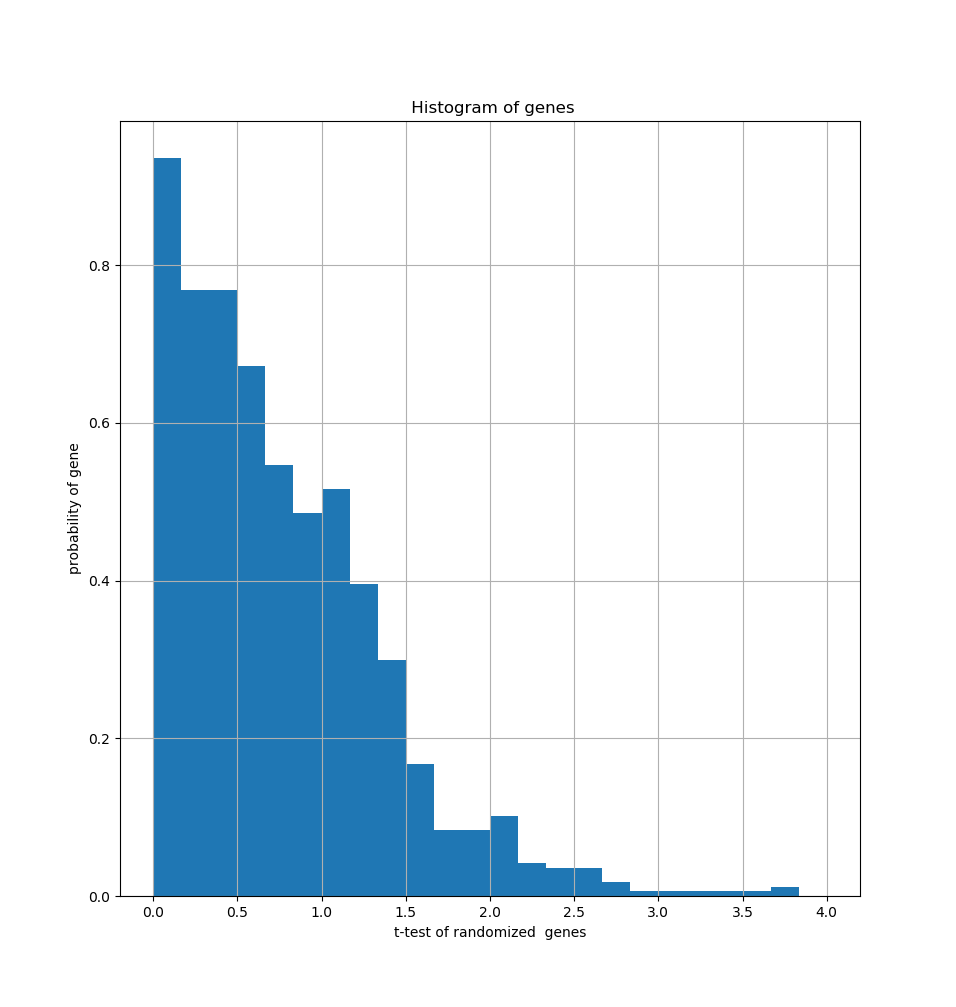
\includegraphics[width=\linewidth]{./Figure1.png}
		\caption{A one side permutantion test with a graphical reperesntation of a bell-like curve.}
		\label{fig:graph1}
		\end{figure}
		 This graph \ref{fig:graph1} show that the absolute value when taken as the first number.

\part{2.E}
 So with with the permuatation data that I randomly shuffled around I was able to get much more closer to the .05 precent with a few tweaks to the intial values. Unforunately, my numbers do randomly shift around alot so there is always a chance of obtaining a prefect number,1.962, because the value will variey 1.565 p-value closer and then there is also a chance of obtain a 3.765 p-value father away form the table. Another weird thing that i realized about my program is that It more closer to 10000 times rather then a thousand fold.   
	\item
\part{3.A}
This question make no sense because you already gave us the final format of the answer.

\part{3.B }
I had a problem with getting the actual graphing to work but I'm a place at which the graph is stored. In which correspound with a memory address. 
	\item
\part{4.A}
"The genomic comparsion of \textit{BRAC2} and \textit{BCR/ABL}  oncegenes with  machines learning algorthims an the abiltiy to find simlarites and  dissimilarities with the regulation of these two genes."
\part{4.B}
		\begin{itemize}
			\item{1}
				Secondary mutations as a mechanism of cisplatin resistance in BRCA2-mutated cancers 
				It show secondary charactistic of BRCA-2 Mutatition 
			\item{2}
				BCR/ABL: from molecular mechainsims of leukemia induction to treatment fof chronic myelogenous leukemia 
				this talks about possible treatments that used to to cure the inferon-\mathrm{\aplha}.
			\item{3}
				Down-regulation of BCRA1 in BCR-ABL-expressing hematopoietic cells

				This article, so that there are breakdown in repairing the protien with a DNA-dependent protine kinase catalytic subunit.
			\item{4}
				Accurate prediction of BRCA1 and BRCA2 heterozygous genotype using expression profiling after induced DNA damage.
				This artcile is the one in which I can start by compare the result of other studies in cancer and try and figure out what happens when you use svm.
		\end{itemize}
\part{4.C}
 
	\item
\part{5}
\end{itemize}
\end{document}    
  

